\def\TheFile{ch05_codelisting.tex}
\begin{savequote}[15cm]
  \vspace{-30mm}
  \sffamily\raggedleft
  Use the source Luke.
  \qauthor{The most accurate documentation is in the source.}
\end{savequote}

\chapter{Listings and Code Documentation}
\label{chap:listings}
Just as much as you can have bad style when including diagrams, the same can happen if
you want to show code snippets.

\begin{Itemize}
\item {\color{red!60!black}\Huge{}NEVER} use screenshots from your IDE and even less so, screenshots with a dark theme.
  Typically your report is read on a white background and the contrast with dark themes is really really bad.
\item In the times you had to print your report I would ask the student who soaked the page with black ink.
\item Big diagrams tend to produce big files and hence also humongous pdf files.
\end{Itemize}

\begin{figure}
  \caption{Bad, Bad way to show quality code}
  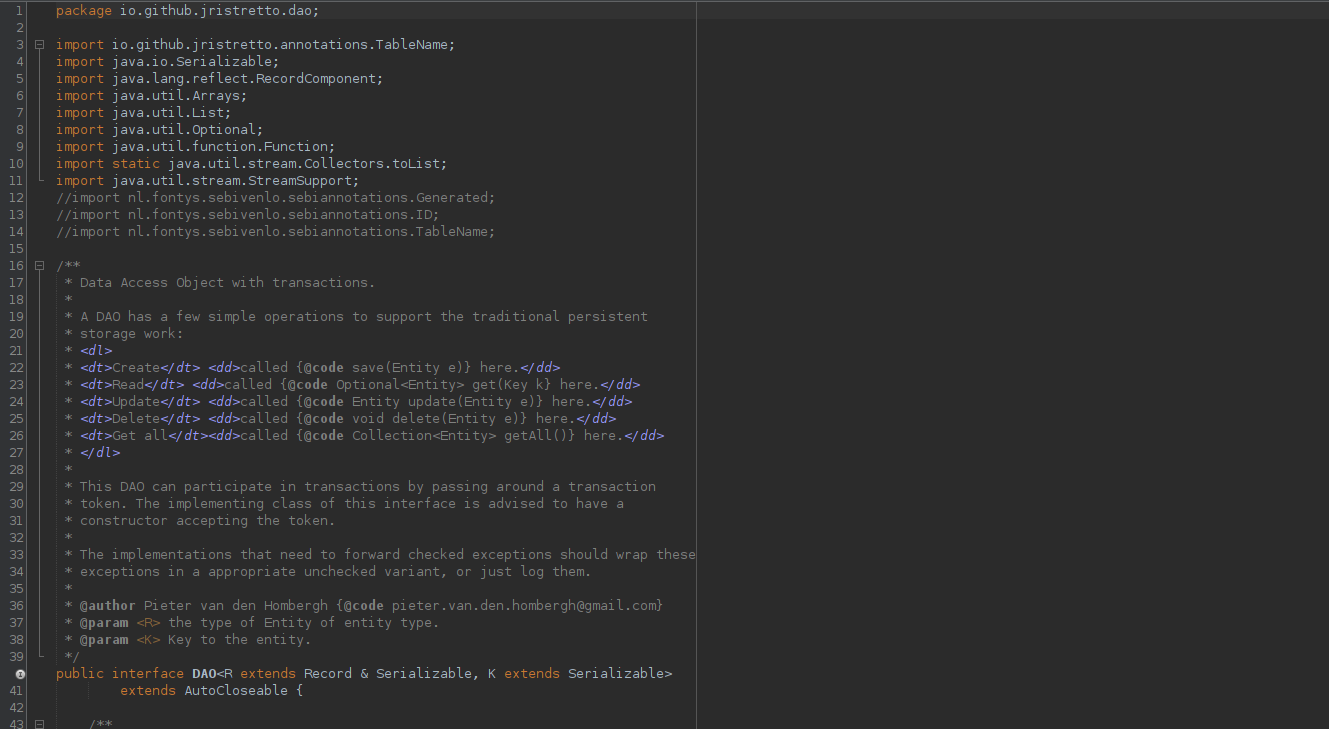
\includegraphics[width=\textwidth]{images/dao.png}
\end{figure}

For these functions to work you need to use the \texttt{package} listings.

\lstset{%first some settings
  numbers=right, % number the lines
  numberstyle={\tiny\color{gray}},frameround=tttt,framerule=1pt,rulesepcolor=\color{gray},
  framexrightmargin=5mm
}

Note that the line numbers in the right hand border are the line
numbers in the included sources.

%% A good advice is to start using \define{doxygen} for your code documentation.
%% It can produce nicely formatted HTML and latex documents and can be
%% tuned in various ways with the  
%% help of doxywizard. The way of working is a lot like using javadoc,
%% but also works for C and C++ files. 
%% See e.g. the documentation on the zthreads package at
%% \url{http://zthread.sourceforge.net} or Qt at 
%% \url{http://doc.trolltech.com/3.3/index.html}

\section{Source code}
The most simple case: include the whole thing with a command like \\
\verb#\lstinputlisting[language=java]{code/Hi.java}#
\lstinputlisting[language=java,caption={Mandatory first program}]{code/Hi.java}

Sometimes it is useful to include just a part of a file, for instance
when you want to explain things. Like what line 11 is all about.\\
\verb#\lstinputlisting[language=java, firstline=11,lastline=11]{Hi.java}#
\lstinputlisting[language=java, firstline=11,firstnumber=11,frame=none,
        lastline=11,numbers=right,basicstyle={\small\ttfamily},
        caption={this is the start of a Java program.}
        ]{code/Hi.java}


The snippet below shows similar code as the snippet above.
And again, you can zoom in and select text.

\lstinputlisting[language=java, firstline=1,firstnumber=1,
        lastline=39,numbers=right,basicstyle={\tiny\ttfamily},
        caption={The proper way to show your code.\label{lst:proper}}
        ]{code/DAO.java}


%% \section{Makefiles}
%% You can also include make files.
%% Note that makefiles have a peculiar syntax. \define{Spaces and tabs in
%%   Makefiles}\ are meaningful. 
%% That's why I made them show up in the next listing with the command\\
%% \lstinputlisting[firstline=65,lastline=67]{chapters/ch05_codelisting.tex}
%% \lstset{showspaces=true,showtabs=true}
%% Spaces show up as \lstinline| |, tab characters as an extended version
%% of the same thing (\lstinline|	|). 
%% As can be expected, spaces and tabs have no special meaning in
%% makefile comments, the lines starting with a hash (\#) sign. 
%% If you want to know more on makefiles try google or info:make in
%% konqueror on a decently installed Linux box.  

%% The make file for this entire document looks like this:
%% \lstinputlisting[language=make,showtabs=true,
%%      showspaces=true,basicstyle={\ttfamily\scriptsize},
%%      numbers=right,language=make]{Makefile}


%%% Local Variables: 
%%% mode: latex
%%% TeX-master: "main"
%%% End: 
